% \pagebreak[4]
% \hspace*{1cm}
% \pagebreak[4]
% \hspace*{1cm}
% \pagebreak[4]
\chapter{ Cài đặt hệ thống } \label{result}

\ifpdf
    \graphicspath{{KetQua/Chapter1Figs/PNG/}{DesignAnalysis/Chapter1Figs/PDF/}{KetQua/Chapter1Figs/}}
\else
    \graphicspath{{Ketqua/Chapter1Figs/EPS/}{KetQua/Chapter1Figs/}}
\fi


\section{Use case sử dụng}

Dựa vào chức năng mà hệ thống sẽ xây dựng sẽ cung cấp, người dùng sẽ có các ca sử dụng như sau:

\begin{figure}[H]
  \begin{center}
    %\leavevmode
    \ifpdf
      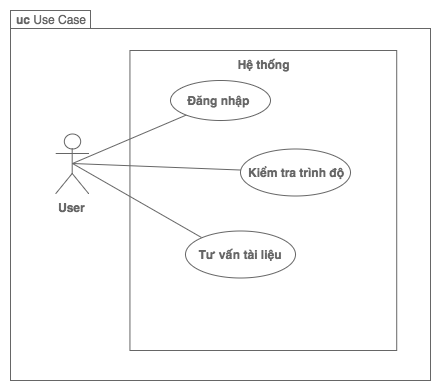
\includegraphics[scale=0.9]{use_case_diagram}
    \else
      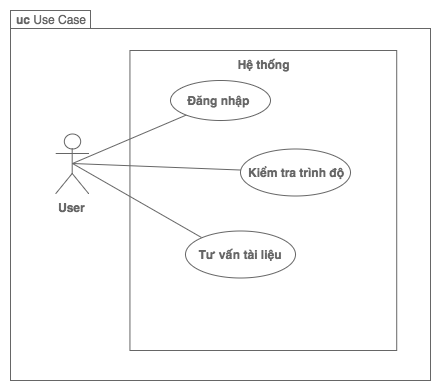
\includegraphics[scale=0.9]{use_case_diagram}
    \fi
    \caption{Use case tổng quan của người dùng}
    \label{Usecase}
  \end{center}
\end{figure}

\begin{table}[H]
\begin{center}
\begin{usecase}
	\addtitle{UC\#001}{Đăng nhập}
	\addfield{Miêu tả}{Người dùng kết nối tài khoản Facebook để đăng nhập vào hệ thống. Nếu tài khoản đăng nhập lần đầu tiên, thông tin người dùng sẽ được khởi tạo trên Firebase} 
	\additemizedfield{Đối tượng}{\item Người dùng}
    \addscenario{Diễn biến chính}{
    \item Người dùng tap vào nút đăng nhập bằng Facebook
    \item Facebook trả về token đăng nhập, hệ thống gửi token lên server Firebase để kiểm tra
    \item Firebase trả về thông tin người dùng 
    \item Hệ thống chuyển đến màn hình chính}
    \addalternative{Diễn biến ngoại lệ}{
    	\item[]3a.  Hệ thống không tìm thấy token, xác định người dùng đăng nhập lần đầu tiên, khởi tạo thông tin người dùng và gửi lên Firebase.
    	\item[]3b.  Hệ thống thông báo lỗi kết nối Internet.}
\end{usecase}
\caption{Đặc tả ca sử dụng: Đăng nhập}
\label{UsecaseLogin}
\end{center}
\end{table}

\begin{table}[H]
\begin{center}
\begin{usecase}
	\addtitle{UC\#002}{Kiểm tra trình độ}
	\addfield{Miêu tả}{Người dùng trả lời các câu hỏi hệ thống đưa ra để xác định trình độ hiện tại của mình} 
	\additemizedfield{Đối tượng}{\item Người dùng}
    \addscenario{Diễn biến chính}{
    \item Người dùng chưa thực hiện kiểm tra trình độ sẽ được hệ thống yêu cầu thực hiện bài kiểm tra.
    \item Người dùng tap vào chọn khoảng thời gian từ khi bắt đầu học tiếng Anh.
    \item Hệ thống tính toán trình độ ban đầu đưa ra câu hỏi với trình độ tương ứng cho người dùng.
    \item Người dùng xem câu hỏi và tap vào đáp án mà nghĩ là đúng.
    \item Hệ thống nhận câu trả lời và đánh giá lại trình độ của người dùng.
    \item Hệ thống kiểm tra xem lĩnh vực hiện tại đã đánh giá được chưa, chuyển sang đánh giá lĩnh vực tiếp theo.
    \item Hệ thống kiểm tra xem đã đánh giá toàn bộ các lĩnh vực chưa, hiển thị kết quả đánh giá trình độ từng lĩnh vực và tổng thể cho người dùng
    }
    \addalternative{Diễn biến ngoại lệ}{
    	\item[]6a.  Chưa đủ để đánh giá trình độ, quay lại bước 3
    	\item[]7a.  Chưa đánh giá hết, chuyển sang đánh giá lĩnh vực tiếp theo, quay lại bước 3}
\end{usecase}
\caption{Đặc tả ca sử dụng: Kiểm tra trình độ}
\label{UsecaseTest}
\end{center}
\end{table}

\begin{table}[H]
\begin{center}
\begin{usecase}
	\addtitle{UC\#003}{Tư vấn tài liệu}
	\addfield{Miêu tả}{Người dùng miêu tả nguyện vọng của họ, các tài liệu sẽ được tư vấn dựa trên trình độ và nguyện vọng đó, người dùng sau đó sẽ đánh giá các kết quả tư vấn và hệ thống sẽ phân tích đưa ra các kết quả tiếp theo phù hợp với cá nhân người dùng} 
	\additemizedfield{Đối tượng}{\item Người dùng}
    \addscenario{Diễn biến chính}{
    \item Người dùng tap vào nút bắt đầu tư vấn.
    \item Hệ thống chuyển sang màn hình hỏi nguyện vọng người dùng.
    \item Người dùng nhập nguyện vọng về tài liệu học tiếng Anh  vào ô nhập liệu.
    \item Hệ thống tính toán và lần lượt đưa ra từng kết quả một dựa trên trình độ và nguyện vọng của người dùng. 
    \item Người dùng đánh giá kết quả tư vấn, di chuyển thanh đo ở từng tiêu chí và tap vào nút đánh giá sau khi hoàn thành
    \item Hệ thống nhận kết quả đánh giá và cập nhập các tiêu chí ưu tiên đối với người dùng.
    \item Kiểm tra xem còn kết quả tư vấn chưa hiển thị hay không, quay trở lại bước 3
    }
    \addalternative{Diễn biến ngoại lệ}{
    	\item[]4a.  Hệ thống không tìm thấy tài liệu phù hợp, thông báo ra màn hình "Không tìm được kết quả phù hợp".
    	\item[]7a.  Không còn kết quả chưa hiển thị, hệ thống chuyển về màn hình chính}
\end{usecase}
\caption{Đặc tả ca sử dụng: Tư vấn tài liệu}
\label{UsecaseRecommend}
\end{center}
\end{table}

\section{Cài đặt hệ thống}
\subsection{Môi trường cài đặt hệ thống}
\begin{itemize}
	\item Hệ điều hành: OS X El Capitan.
	\item Môi trường phát triển: Android Studio
	\item Cơ sở dữ liệu: SQLite, Firebase.
	\item Framework: Android SDK.
	\item Ngôn ngữ: Java.
\end{itemize}
\subsection{Kiến trúc hệ thống cài đặt}

Kiến trúc hệ thống cài đặt được mô tả như hình vẽ dưới đây:\\

\begin{figure}[H]
  \begin{center}
    %\leavevmode
    \ifpdf
      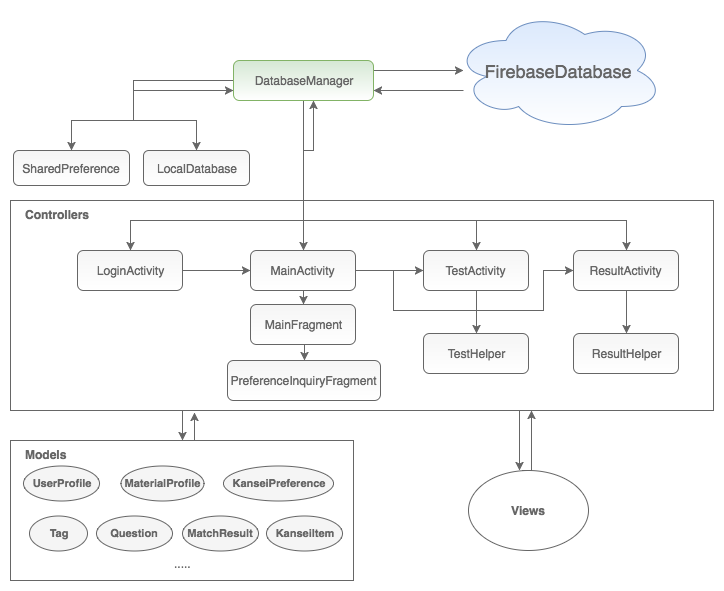
\includegraphics[scale=0.65]{system_diagram}
    \else
      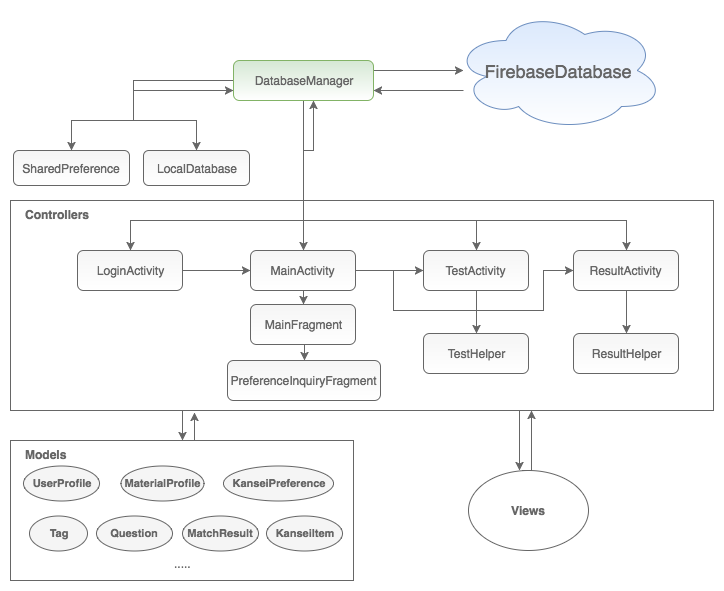
\includegraphics[scale=0.65]{system_diagram}
    \fi
    \caption{Mô hình kiến trúc hệ thống}
    \label{SystemDiagram}
  \end{center}
\end{figure}

Các thành phần chính của hệ thống:

\begin{itemize}
	\item \textbf{FirebaseDatabase: }Lớp Wrapper của Firebase SDK trên Android, có nhiệm vụ kết nối với cơ sở dữ liệu thời gian thực Firebase Realtime Database và thực hiện các câu lệnh truy vấn đến Database cũng như trả kết quả từ Firebase về client Android.
	\item \textbf{DatabaseManager: }Lớp quản lý truy xuất dữ liệu sử dụng trong hệ thống, đóng vai trò cầu nối giữa Controller và Firebase, đặc tả các câu lệnh truy xuất dữ liệu, gửi đến Server và xử lý kết quả trả về từ Json về các Model đã định nghĩa. Ngoài ra, lớp này còn đóng vai trò giao tiếp với Local Database và Shared Preference để gửi và nhận dữ liệu lưu trữ trên thiết bị. 
	\item \textbf{LocalDatabase: } Cơ sở dữ liệu địa phương, copy và lưu trữ dữ liệu ở Firebase sau lần truy xuất lấy dữ liệu đầu tiên. Ở các lần khởi động hệ thống tiếp theo, một truy vấn sẽ được gửi đến Firebase xem bộ dữ liệu có thay đổi gì không, cập nhập bộ dữ liệu địa phương nếu có phát hiện thay đổi, đảm bảo đồng bộ giữa client và server.
	\item \textbf{SharedPreference: } Lưu trữ thông tin đăng nhập của người dùng sau lần đăng nhập đầu tiên. Người dùng sẽ được tự động đăng nhập vào hệ thống vào các lần khởi động ứng dụng tiếp theo.
	\item \textbf{Controllers: } Bao gồm các lớp thực hiện điều khiển và thực hiện các tác vụ chính trong hệ thống. Controller bắt các tương tác từ người dùng với giao diện đặc tả ở View và xác định yêu cầu, gọi các phương thức để xử lý chúng sau đó hiển thị kết quả lên giao diện người dùng. Mỗi Activity ( và Fragment ) đi kèm với chúng đóng vai trò thực hiện một tác vụ nhất định trong hệ thống, nằm giữa giao tiếp với Model và View. Ngoài ra, các lớp Helpers đóng gói các phương thức xử lý logic phức tạp, cài đặt thuật toán thực hiện trong hệ thống.   	
	\item \textbf{Models: } Bao gồm các lớp chứa dữ liệu được tổ chức có cấu trúc, mỗi lớp đặc trưng cho một đối tượng cụ thể mà Controller hoặc các thành phần khác sẽ gọi đến để sử dụng trong xử lý bài toán. Dữ liệu lưu trữ trong cơ sở dữ liệu đều được lưu dưới dạng các đối tượng của lớp Model.
	\item \textbf{Views: } Bao gồm các file .xml đặc tả cấu trúc, cách bố trí và sự xuất hiện của giao diện ứng dụng, trong đó có layout, drawable, animation, value về màu sắc, style, font chữ ..v..v...Mỗi Activity và Fragment sẽ có một layout tương ứng với chúng.	 
\end{itemize}

\subsection{Biểu đồ lớp theo ca sử dụng}

\begin{figure}[H]
  \begin{center}
    %\leavevmode
    \ifpdf
      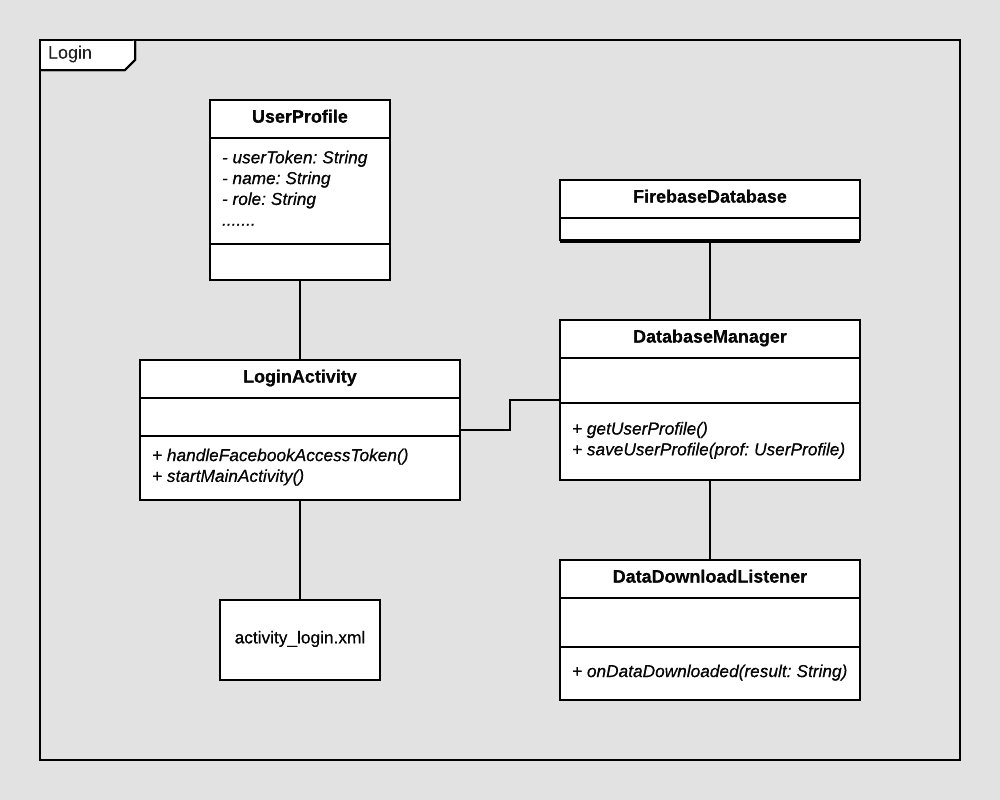
\includegraphics[scale=0.92]{class_login}
    \else
      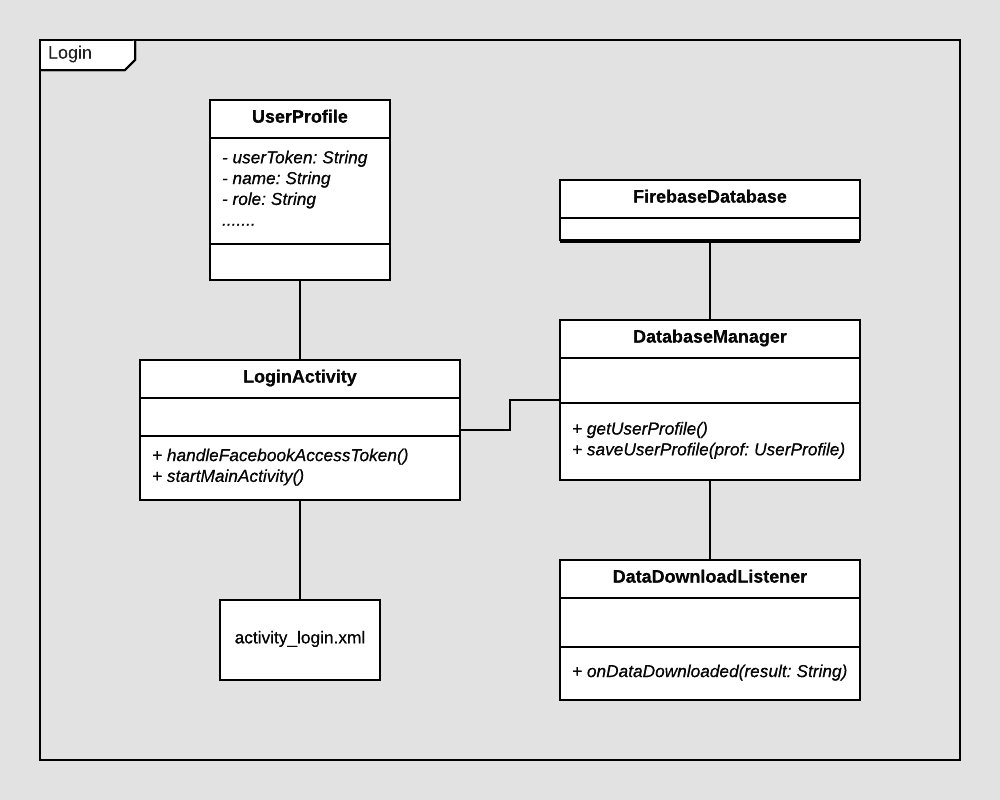
\includegraphics[scale=0.92]{class_login}
    \fi
    \label{LoginClassDiagram}
    \caption{Biểu đồ lớp theo ca sử dụng: đăng nhập}
  \end{center}
\end{figure}

\begin{figure}[H]
  \begin{center}
    %\leavevmode
    \ifpdf
      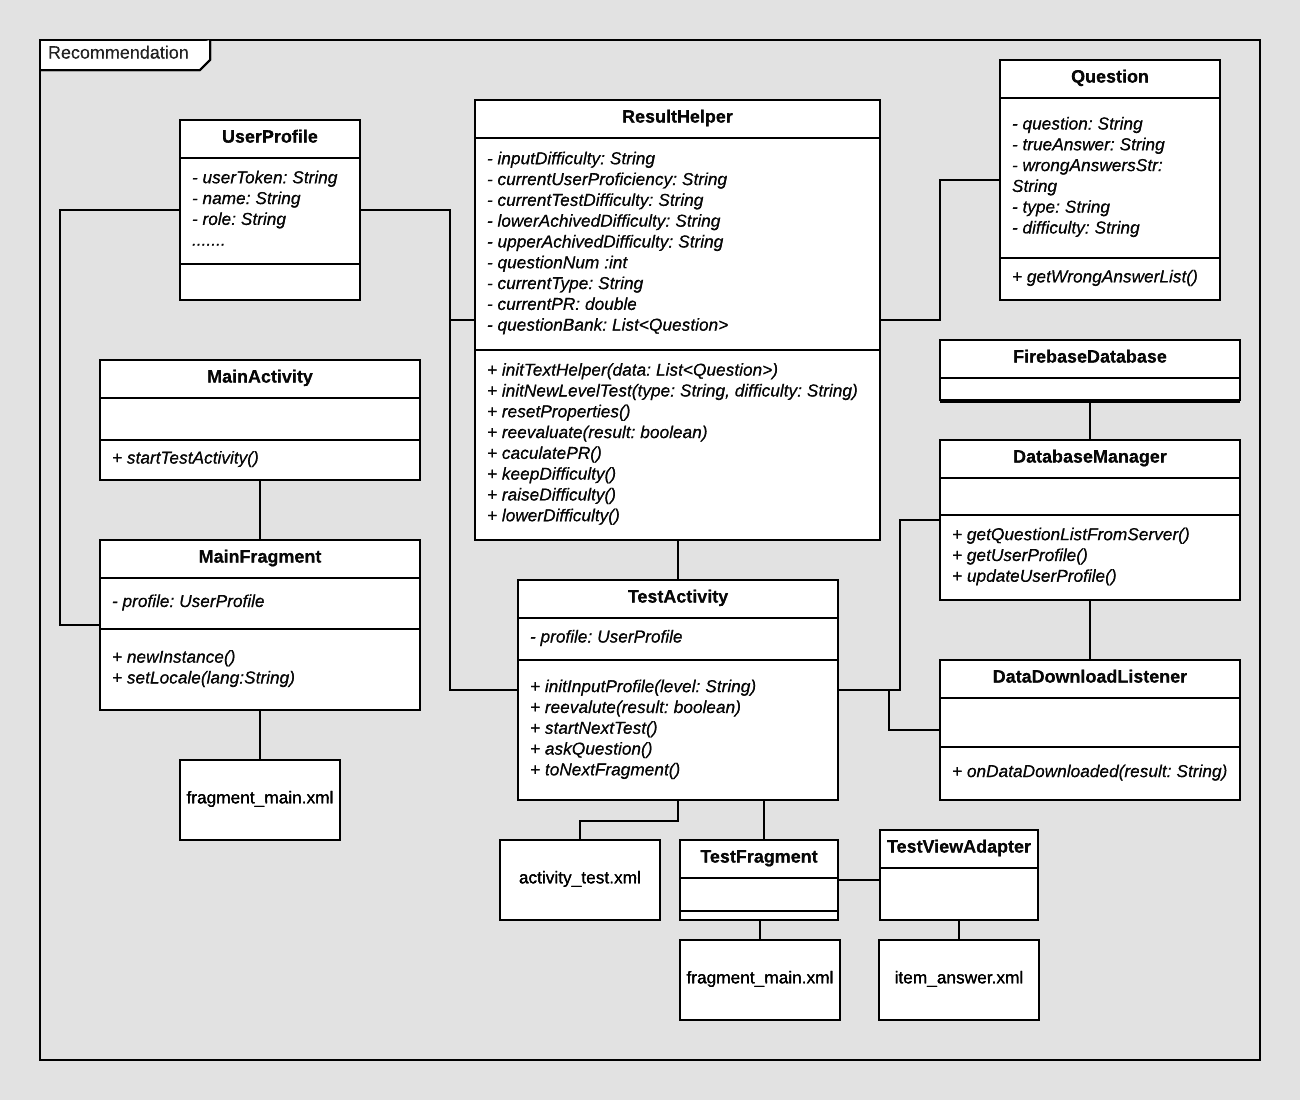
\includegraphics[scale=0.8]{class_testprof}
    \else
      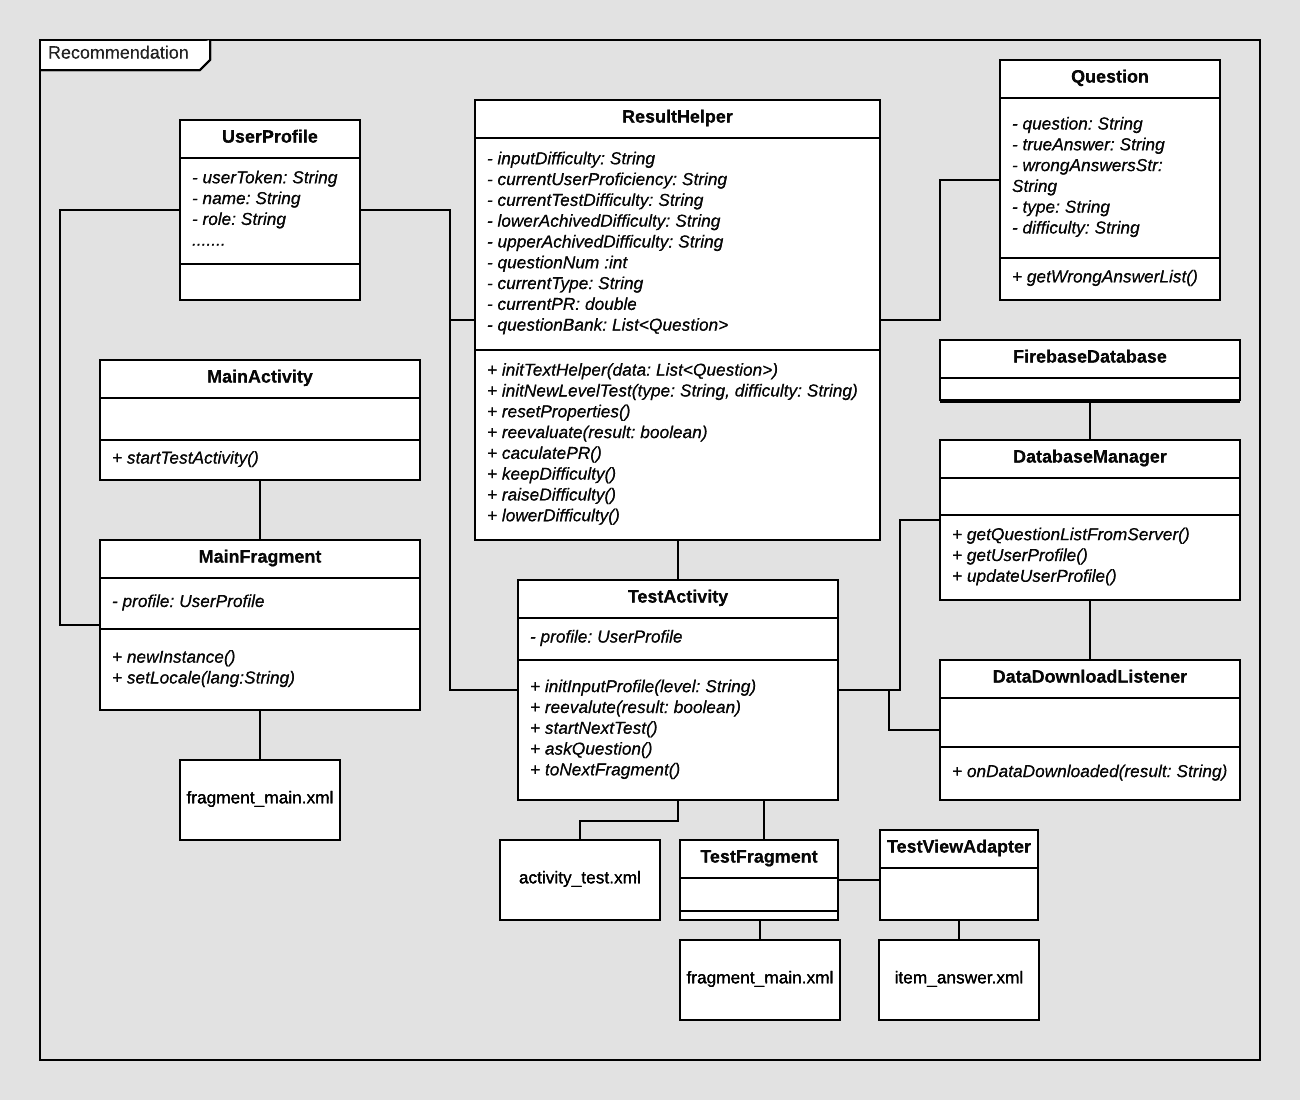
\includegraphics[scale=0.8]{class_testprof}
    \fi
    \label{TestProficiencyDiagram}
    \caption{Biểu đồ lớp theo ca sử dụng: kiểm tra trình độ}
  \end{center}
\end{figure}

\begin{figure}[H]
  \begin{center}
    %\leavevmode
    \ifpdf
      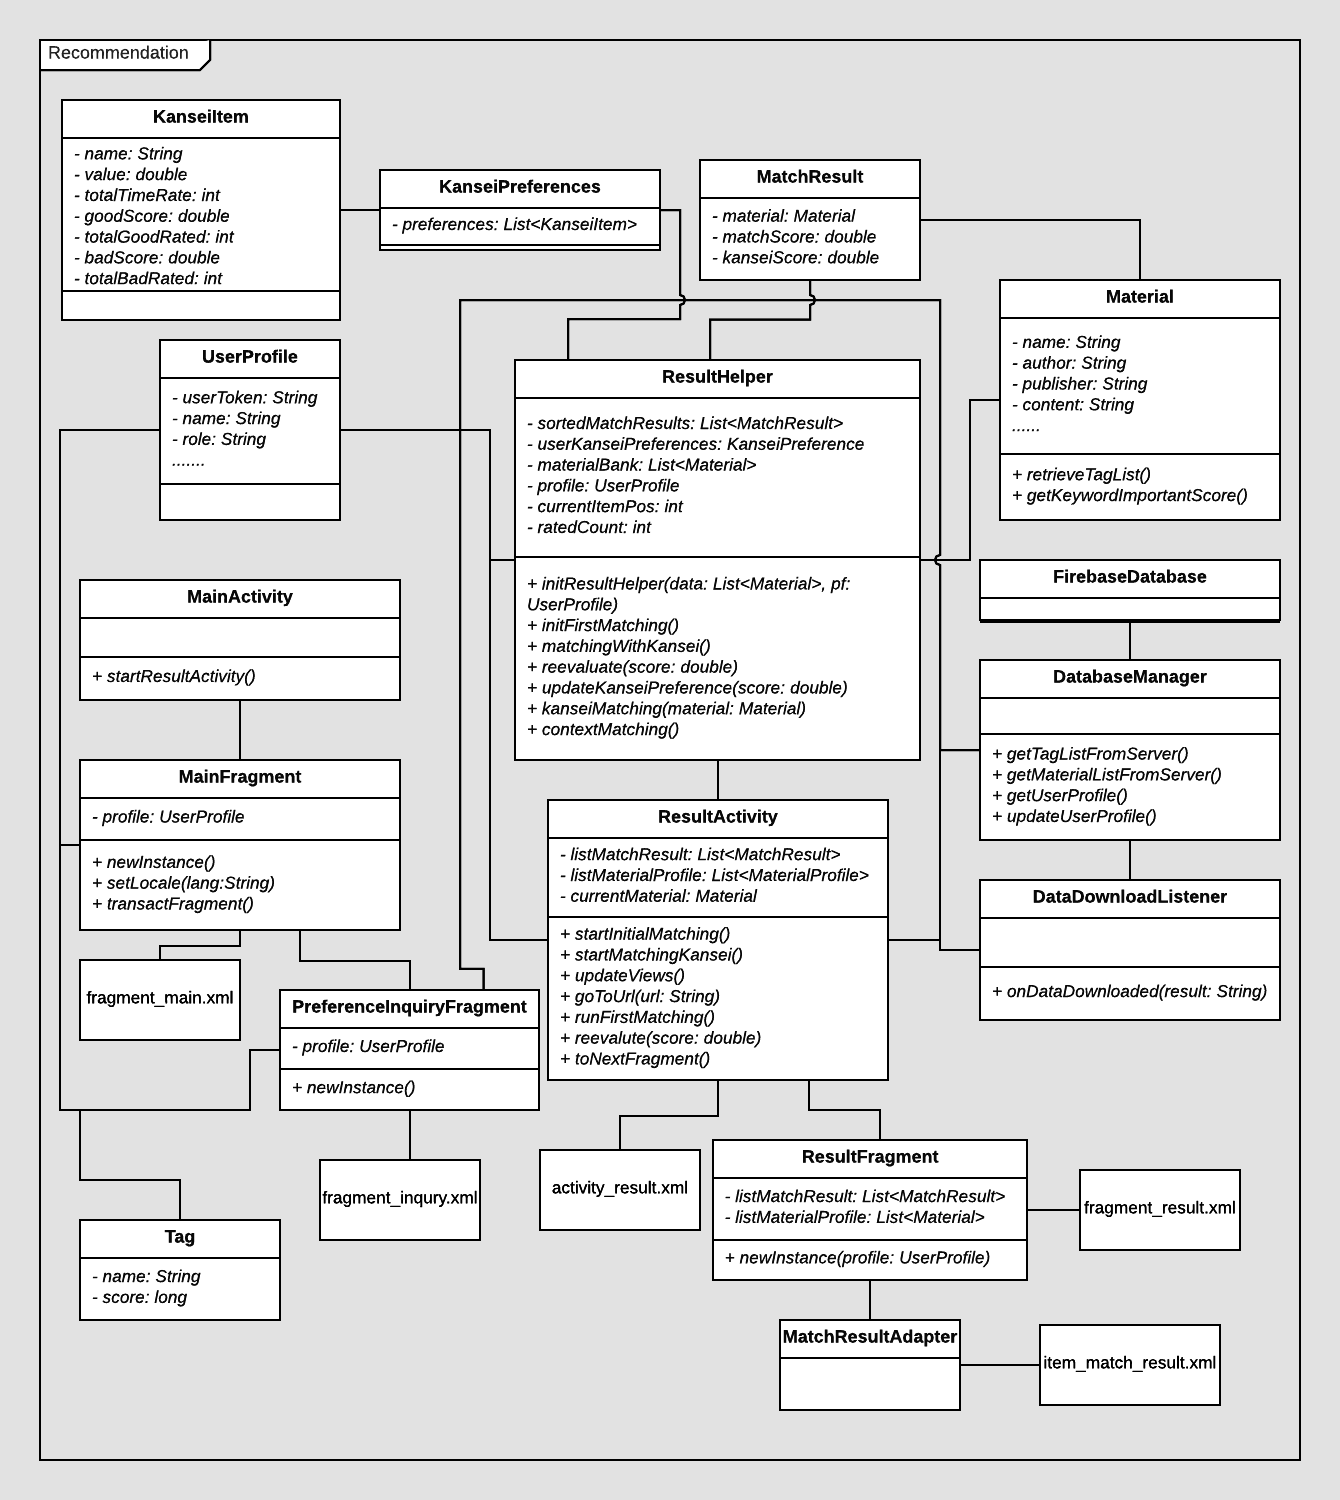
\includegraphics[scale=0.8]{class_recommendation}
    \else
      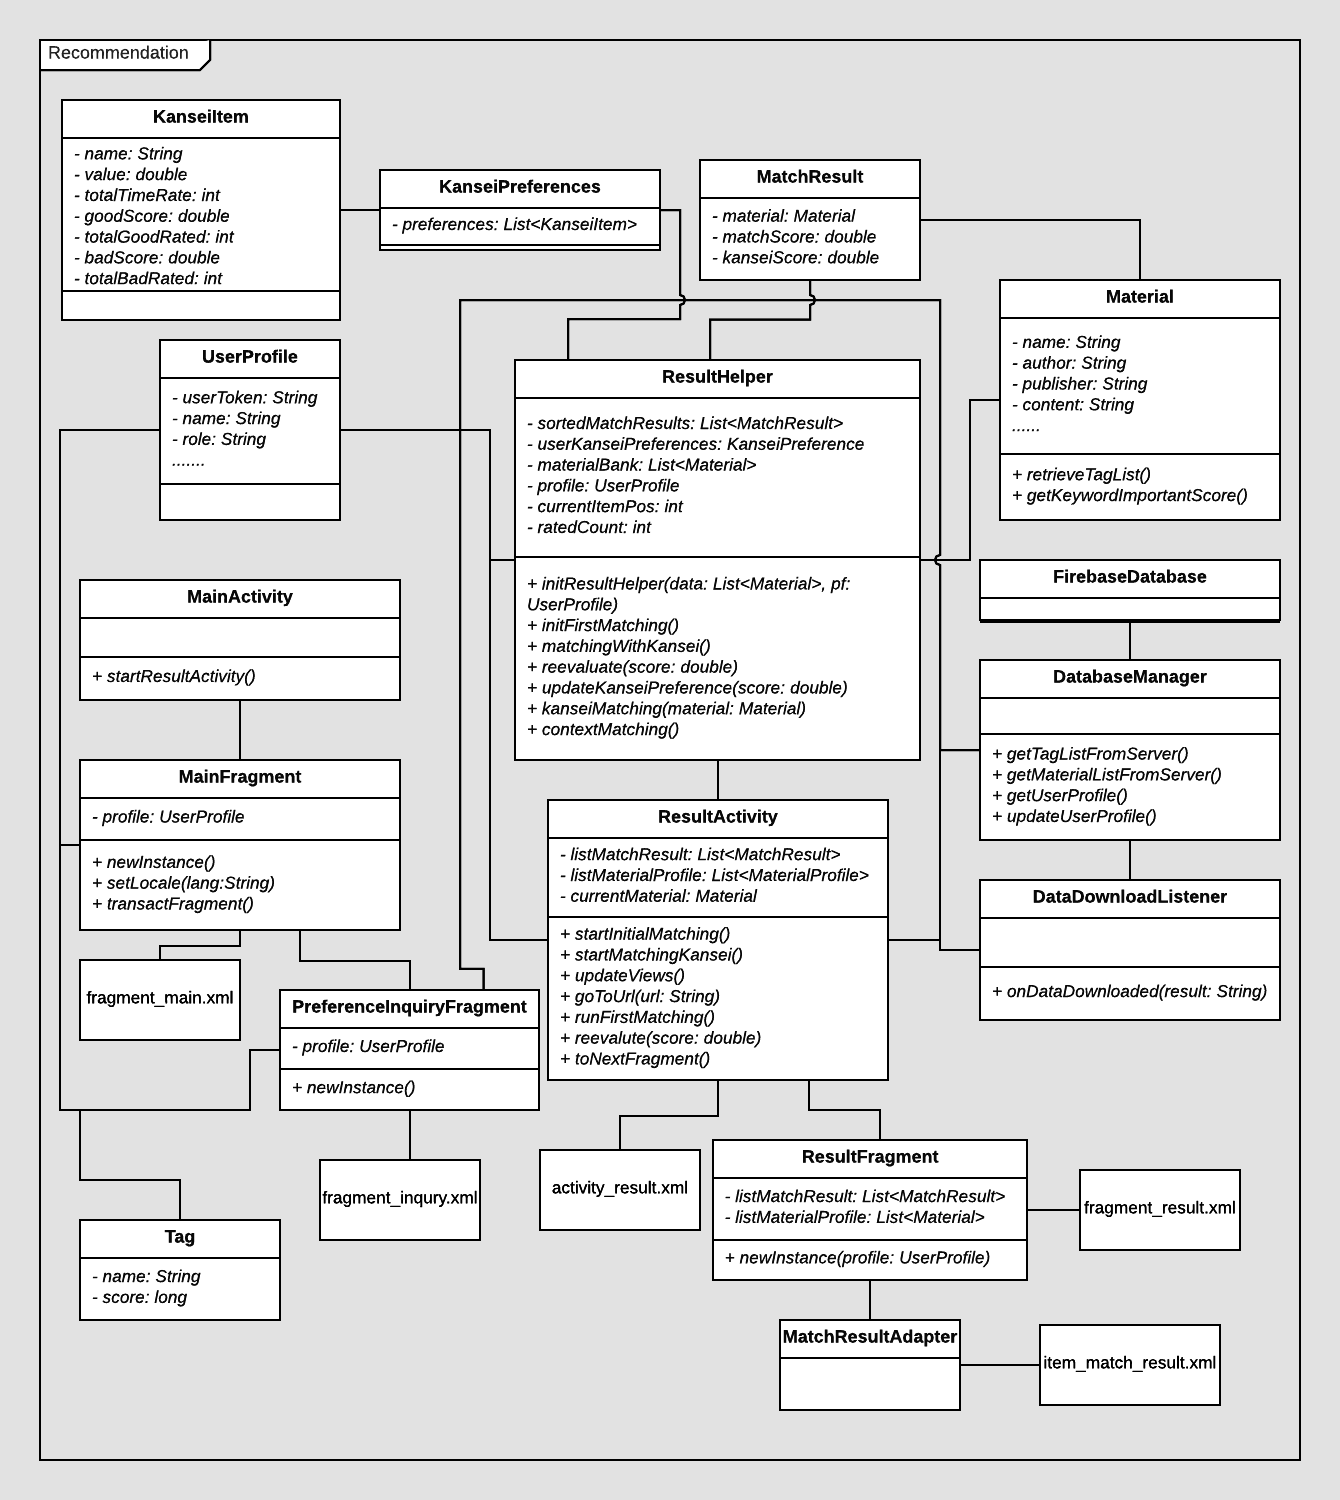
\includegraphics[scale=0.8]{class_recommendation}
    \fi
    \label{RecommendationDiagram}
    \caption{Biểu đồ lớp theo ca sử dụng: tư vấn tài liệu}
  \end{center}
\end{figure}

\subsection{Mô hình cơ sở dữ liệu}

Dữ liệu lưu trữ trên Firebase được lưu trữ dưới dạng NoSQL, khác với các mô hình RDBMS thông thường. Trong NoSQL, dữ liệu được lưu trữ dưới dạng JSON, mô hình dưới dạng mà hệ thống có thể sử dụng trực tiếp, loại bỏ các ràng buộc liên kết giữa bảng với bảng. Các thuộc tính trong một đối tượng được trải đều ra và không khuyến khích phân tầng, truy xuất dựa trên các cặp "key" và "value". Nhờ vậy, NoSQL cho ra hiệu năng cao hơn khi cần truy xuất tập dữ liệu lớn so với các mô hình RDBMS thông thường.


\begin{figure}[H]
  \begin{center}
    %\leavevmode
    \ifpdf
      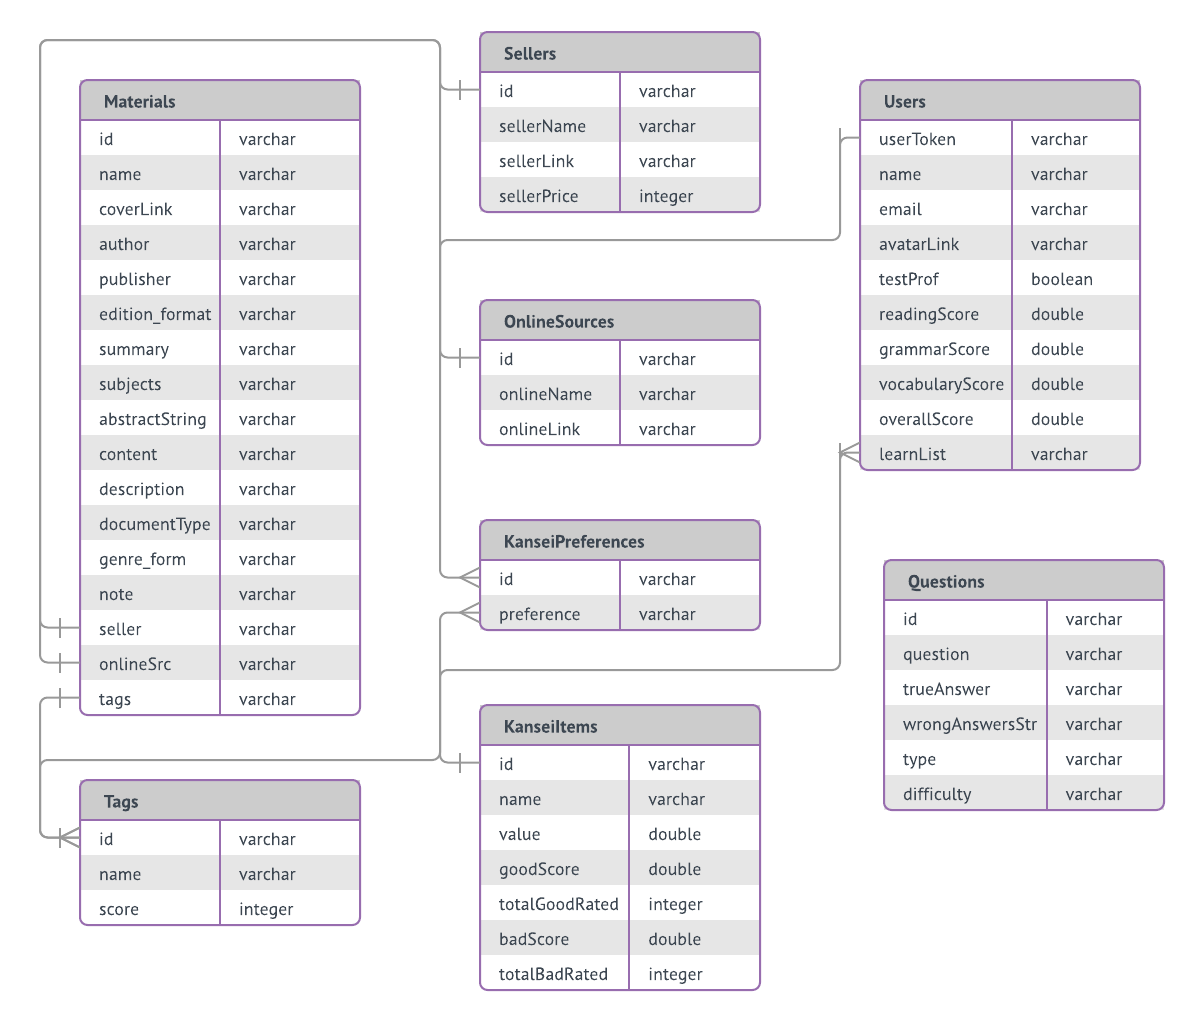
\includegraphics[scale=0.58]{database_diagram}
    \else
      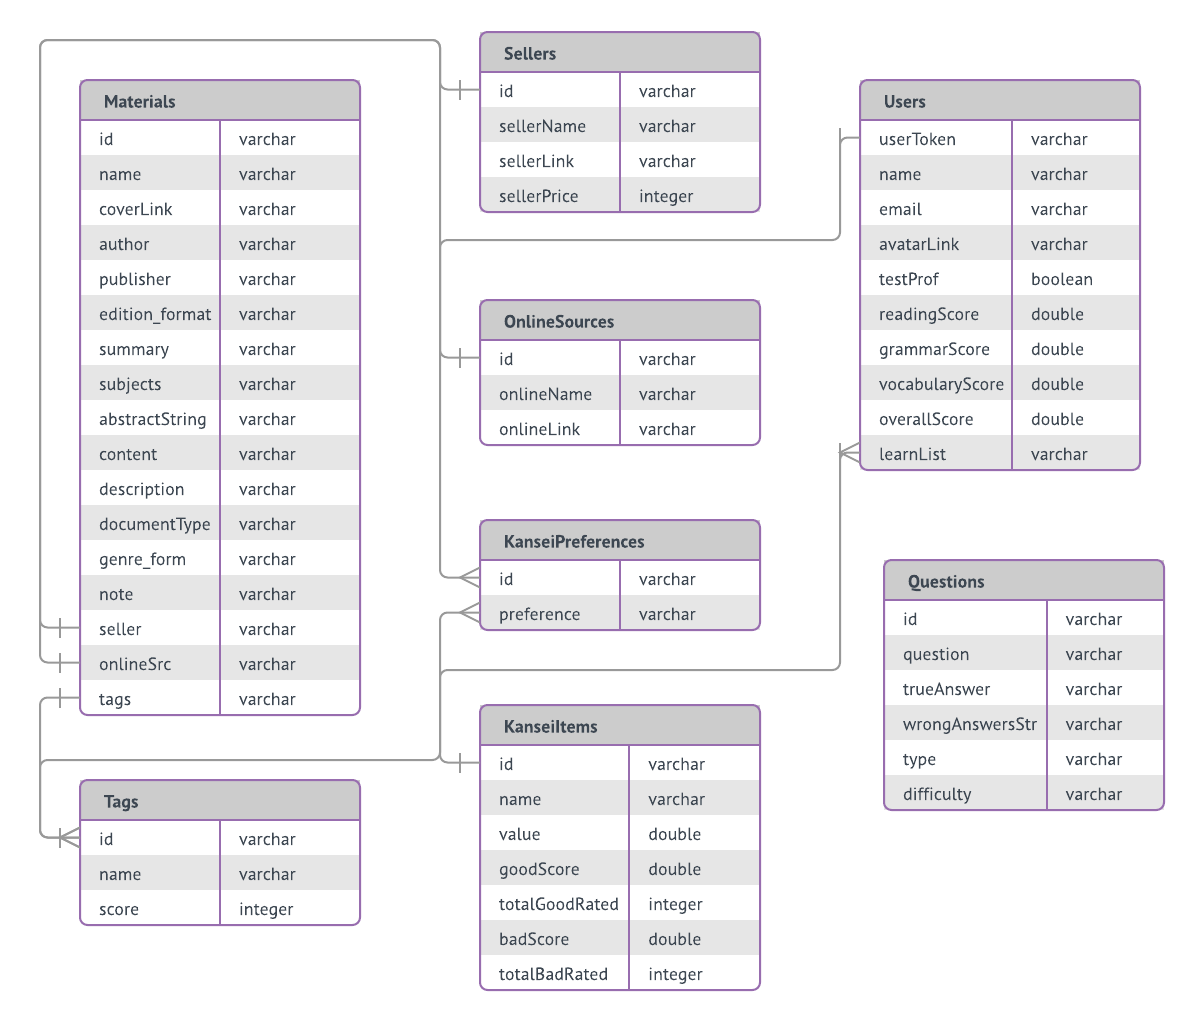
\includegraphics[scale=0.58]{database_diagram}
    \fi
    \caption{Mô hình cơ sở dữ liệu}
    \label{DatabaseDiagram}
  \end{center}
\end{figure}


\section{Kết quả cài đặt}

2

